\section{Distance Estimation}\label{distance-estimation}\index{distance estimation}

Distance Estimation (DE) is the calculation of an estimated distance from the
given point to the nearest surface of the fractal. As suggested by the word
'estimate', it is an approximate value. It is calculated using simplified
algorithms based on analytical (Analytical DE)\index{distance estimation!analytical} or numerical (Delta DE)\index{distance estimation!delta DE}
calculations of gradients.

DE is the most important algorithm required to render three-dimensional fractals
within a reasonable time. It achieves a great reduction in the number of steps
needed to find the exact area of the fractal while tracking a ``photon''
traveling toward the object along a ray (a simulated beam of light from the
camera eye). A ray is generated for each pixel (1000 x 1000 resolution =
1,000,000 rays). They match FOV from the camera eye (i.e. they are not
parallel.)

Without the DE calculation, the proximity of the photon to the fractal surface
would need to be repeatedly calculated after each of many very small steps. For
example, without an estimate of where the fractal surface is, you may need up to
10,000 steps to trace a ray of light, for every pixel of the image.

Using DE, the size of the steps along the ray of light can be increased, based
on the calculated estimate of where the fractal surface should approximately be
located. The process of moving along the ray and testing for the surface
location is called ray-marching.

Ray marching\index{ray marching} looks like the illustration below. In each step, an estimation on
the distance to the nearest fractal surface is calculated. The photon is moved
along the ray by this distance. The next step is re-calculated based on the
estimated distance. This distance is less so this time the Photon is moved a
smaller distance. The ray-marching becomes more accurate closer to the surface
of the fractal. The ray marching ceases when the photon becomes within a set
``distance threshold''\index{ray marching!distance threshold} from the surface or after a maximum number of iteration
if the option ``stop at maximum iteration'' is enabled.

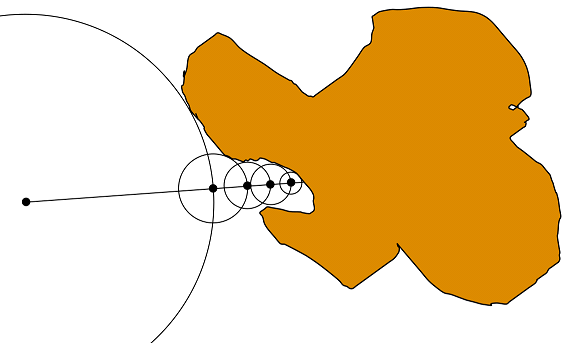
\includegraphics[width=0.7\linewidth]{img/manual/media/distance_estimation_defactor_1.png}

Since the estimation contains some error (sometimes quite large), there is a
risk that the step of moving the "photon" will be too large, and incorrectly it
will flow into the surface of the fractal. This may result in visible noise in
the rendered image.

To prevent this, the "photon" can be moved by the estimated distance multiplied
by a number between 0 and 1 ("ray-marching step multiplier"\index{ray marching!step multiplier}). Steps are then
smaller, so there is less risk of "overshooting" the surface, but the rendering
time increases due to more steps being required.

Below is an example for a step multiplier of 0.5:
\nopagebreak

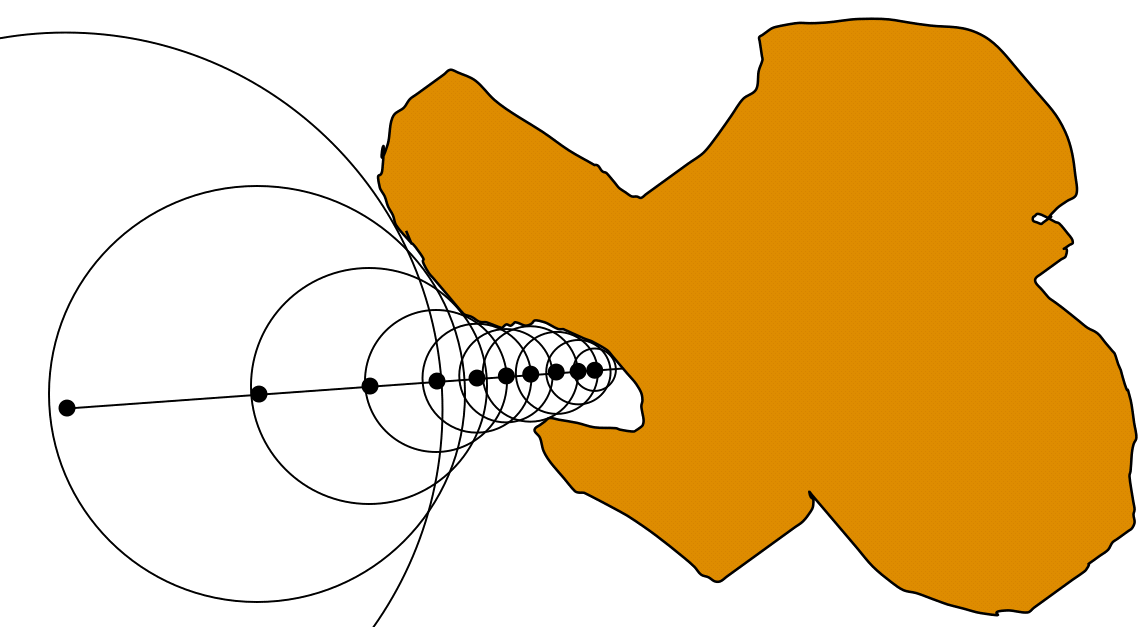
\includegraphics[width=0.7\linewidth]{img/manual/media/distance_estimation_defactor_05}

Raymarching with step multiplier 0.5 produces high iteration count and good DE

Each formula has assigned a DE mode and function (``preferred''). In most cases
the preferred \emph{mode} is \emph{Analytical DE} (fastest).

The preferred \emph{function} is assigned based on whether the formula is
transforming in a linear or logarithmic manner. These setting can be varied on
the \emph{Render Engine} tab.

\emph{Analytical DE}\index{distance estimation!analytical} mode is faster than \emph{Delta DE}\index{distance estimation!delta DE} mode to calculate.
However with some formulas only Delta DE mode will produce a good quality image.
The DE modes can be used with either linear or logarithmic DE functions.

Example linear out: $ distance = \frac{r}{\lvert DE \rvert} $

Example logarithmic: $ distance = \frac{0.5 r  \log(r)}{DE} $

The quality produced by the DE mode and function combinations is formula
specific. The setting of formula parameters can also greatly affect the quality
produced by the DE. In some cases the choice of fractal image is determined by
what location and parameters can produce good DE quality.

Statistics Tab with histogram data\index{statistics!wrong distance estimations}:
\nopagebreak

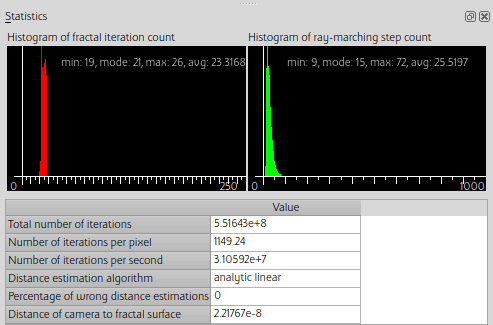
\includegraphics[width=0.7\linewidth]{img/manual/media/dock_statistics.png}

In the Statistics (enable in \emph{View} menu) you can see \emph{Percentage of
	Wrong Distance Estimations} ("Bad DE"). This number is the percentage of image
pixels which potentially have big errors in distance estimation calculation
(estimated distance was much too high). It is visible as a noise on the image.
As a general rule less than 0.1 is good, but it is case specific and 3.0
sometimes is OK and 0.0001 sometimes is not.
